\chapter{Experiments}\label{sec:experiments}

Assessments of the effectiveness of the six scheduler queues  have been conducted using different configurations of the \textbf{PHOLD} benchmark and the \textbf{PCS} simulation. The experiments were conducted on our previously described distributed memory computing cluster. Our initial experimental analysis proved to be time consuming due to the large number of parameters (see Tables~\ref{tab:phold-params} and ~\ref{tab:pcs-params}) and combinations of their values. Consequently, we pursued strategies to focus on the most influential parameters that impacted relative performance of the scheduler queues using Generalized Sensitivity Analysis (GSA)~\cite{guven-07}. 

\section{Parameter reduction via GSA}\label{sec:gsa}

Generalized Sensitivity Analysis (GSA) is based on two-sample Kolmogorov-Smirnov Test (KS-Test) and yields a $d_{m,n}$ statistic
that is sensitive to differences in both central tendency and differences in the distribution functions of
parameters~\cite{guven-07}. The $d_{m,n}$ statistic is the maximum separation between cumulative probability distribution observed in a
two-sample KS-Test. The KS-Test is performed with data from Monte Carlo simulations involving combinations of parameter values from a
specified range or probability distribution. The simulation result is then classified into number of ``success'' ($m$) or its converse
``failure'' ($n$) to compute cumulative probability distribution and $d_{m,n}$ statistic for each parameter. In this study we have defined
``failure'' to be parameter values for which the \textbf{2tLadderQ} runs slower when compared to another scheduler queue. For sequential and parallel simulations we use \textsubscript{t2}\textit{k}=1 and \textsubscript{t2}\textit{k}=128 respectively.

An important aspect of GSA is to ensure that the values for each parameter covers its full range of values. Consequently, we use Sobol
random numbers to select a combination of \textbf{PHOLD} parameter values to be used for simulation. Sobol random numbers are quasi-random
low-discrepancy sequences that provide uniform coverage of a multidimensional parameter space for \textbf{PHOLD} (see Figure~\ref{fig:phold}). Our parameter ranges also ensure that the peak memory consumption do not cross NUMA threshold, which in our case is 4 GB of RAM. Exceeding the 4 GB NUMA threshold introduces a lot of variance in runtimes requiring many runs to reduce variance to acceptable limits.

The randomly (using Sobol sequences) selected parameter set is used to run the model using two different scheduler queues. Average simulation execution time from 3 different replications is recorded for each scheduler queue along with the parameter-set. The process is
repeated for 2,500 different Sobol sequences. The 2,500 data set is then collectively analyzed to compute the $d_{m,n}$ statistics for the
different parameters.

\begin{figure}[H]
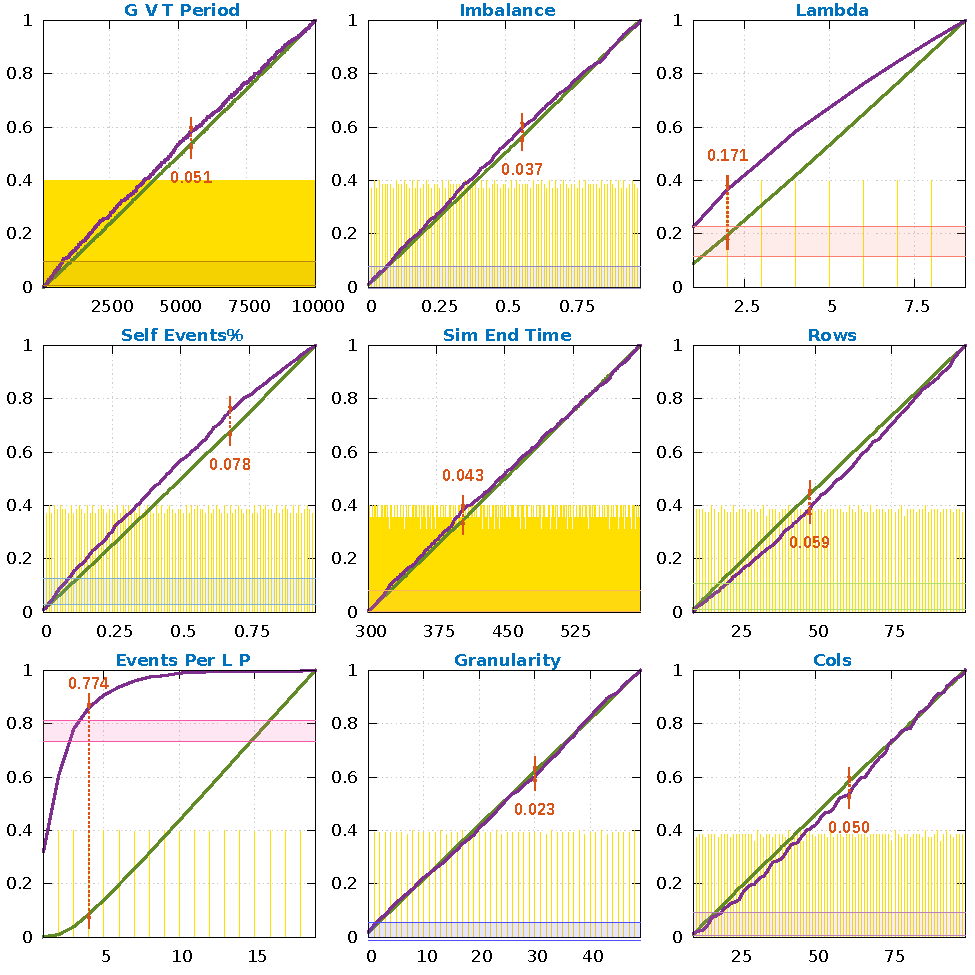
\includegraphics[width=\linewidth]{images/2tlad_vs_3tHeap_gsa}
\textbf{\caption{Results from Generalized Sensitivity Analysis (GSA) comparing \textbf{2tLadderQ and \textbf{3tHeap}} for sequential simulation using the PHOLD benchmark.}\label{fig:gsa-3tvs2t}}
\end{figure}

\subsection{GSA results for sequential simulations using PHOLD}\label{sec:seq-gsa}

The charts in Figure~\ref{fig:gsa-3tvs2t} show the cumulative $m$, $n$, and the $d_{m,n}$ statistics for the 9 different \textbf{PHOLD} parameters
explored using GSA for sequential simulations. The orange impulses show the parameter values and number of samples used for Monte Carlo
simulation. Note that the distribution of samples varies depending on the nature of the parameter -- \textit{i.e.,} \textbf{eventsPerLP} varies in discrete steps of 1 from 1--20 while \textbf{imbalance} varies from 0 to 1.0 in small fractional steps.

\begin{figure}[H]
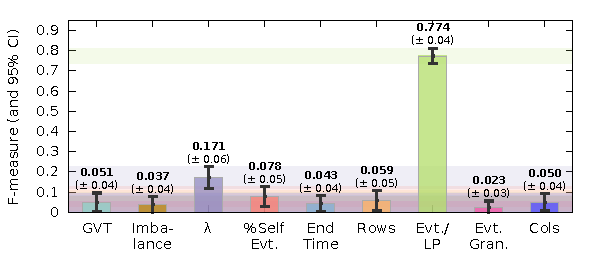
\includegraphics[width=\linewidth]{images/2tlad_vs_3tHeap_gsa_anal_short}\vspace{-0.1in}
\textbf{\caption{Summary of influential parameters from
Figure~\ref{fig:gsa-3tvs2t} that cause performance differences
between \textbf{2tLadderQ} and \textbf{3tHeap} in sequential
simulations using PHOLD.}\label{fig:gsa-anal-3tvs2t}}
\end{figure}

The chart in Figure~\ref{fig:gsa-anal-3tvs2t} shows the summary of the $d_{m,n}$ statistic or influence of each parameter (see Table~\ref{tab:phold-params}) on the outcome -- \textit{i.e.,} \textbf{2tLadderQ} performs better or worse than \textbf{3tHeap}. The lightly shaded bands show the 95\% Confidence Intervals (CI) computed using standard bootstrap approach using 5000 replications with 1000 samples in each. As expected, the \textbf{imbalance} (\textit{i.e.,} skew in partition) has no impact in sequential simulation and has a low impact score of 0.037. Similarly, the GVT computation rate does not impact pending events and consequently its influence is low at 0.051.

Interestingly, other model parameters such as \textbf{rows}, \textbf{cols}, \textbf{self-events}, \textbf{simEndTime}, and \textbf{granularity} have no influence on relative performance of \textbf{2tLadderQ} vs \textbf{3tHeap}. The parameter with most influence is \textbf{eventsPerLP} with a score of 0.774. This parameter determines total number of concurrent events which influences bucket sizes and number of rungs in \textbf{2tLadderQ} as well as the third tier size in \textbf{3tHeap}. The parameter $\lambda$ for exponential distribution has a marginal influence because it influences number of concurrent events as discussed in Section~\ref{sec:pholdModel} and shown in Figure~\ref{fig:phold}(c).

We have also conducted GSA to determine influential parameters impacting performance of other scheduler queues versus the \textbf{2tLadderQ} in sequential simulations. Our analysis showed that none of the parameters play an influential role and the \textbf{2tLadderQ} performed consistently better or the same when compared to \textbf{ladderQ}, \textbf{2tHeap}, \textbf{fibHeap}, and \textbf{heap}. Only \textbf{3tHeap} and in few cases \textbf{2tHeap} outperformed our \textbf{2tLadderQ} in certain configurations.  The performance of \textbf{ladderQ} and \textbf{2tLadderQ} was practically indistinguishable in sequential simulations (with \textsubscript{2t}\textit{k}=1).

\begin{figure}[H]
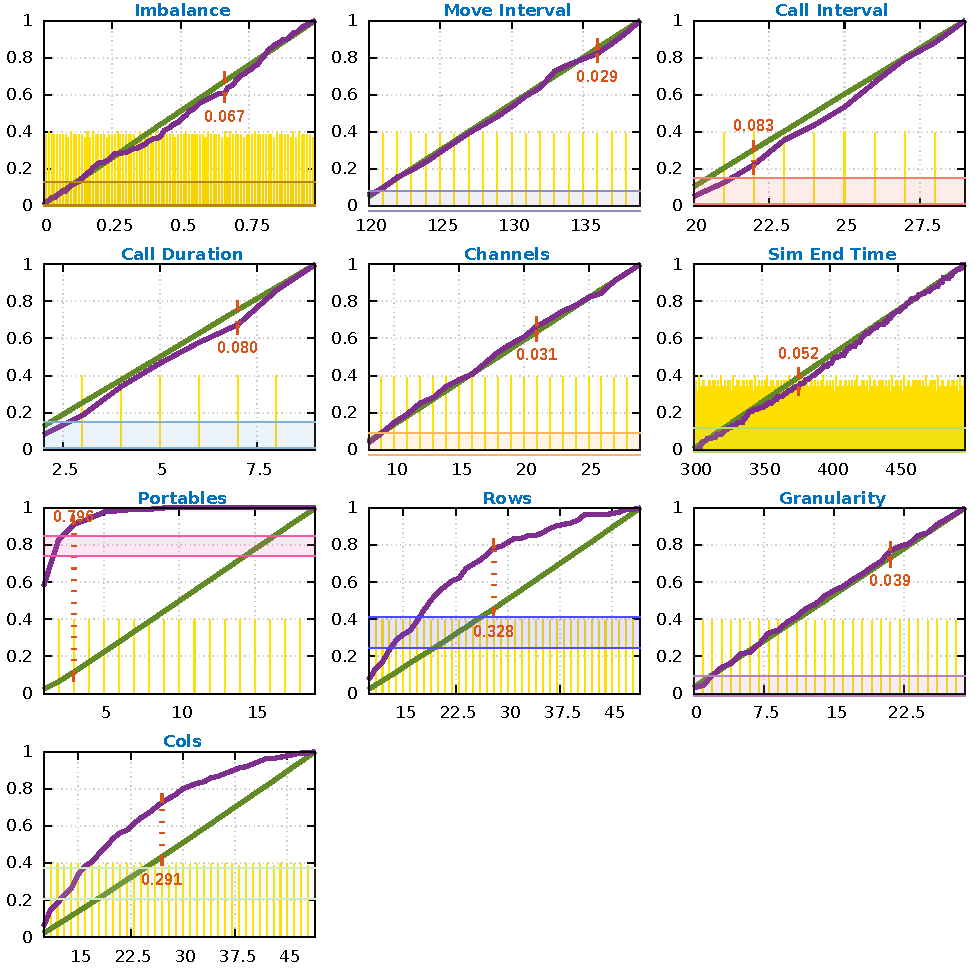
\includegraphics[width=\linewidth]{images/full_gsa_2tladv3tHeapPCS.pdf}
\textbf{\caption{Results from Generalized Sensitivity Analysis (GSA) comparing \textbf{2tLadderQ} and \textbf{3tHeap} for sequential simulation using PCS.}\label{fig:gsa-2tladv3tPCS}}
\end{figure}

\subsection{GSA results for sequential simulations using PCS}\label{sec:seq-gsa-PCS}

The charts in Figure~\ref{fig:gsa-2tladv3tPCS} shows the two-sample KS-Test statistics for the cumulative probability distribution functions of the 10 different \textbf{PCS} parameters. The GSA data shows that in sequential simulations, most of  the parameters do not influence performance difference between \textbf{2tLadderQ} and \textbf{3tHeap} with $d_{m,n}$ << 0.1. As expected \textbf{portables} was the most influential parameter in the simulation. This parameter is equivalent to the \textbf{eventsPerLP} parameter in the \textbf{PHOLD} benchmark. In similarity to the GSA results using \textbf{PHOLD}, higher values of \textbf{portables} parameter cause the \textbf{3tHeap} to perform better than the \textbf{2tLadderQ}. The summary of influential parameters in Figure ~\ref{fig:gsa-anal-2tladv3tPCS} shows the \textbf{portables} parameter with a high impact score of 0.796. In addition, \textbf{rows} and \textbf{cols} parameters displayed marginal influence with low impact scores of 0.328 and 0.291, respectively.   

\begin{figure}[H]
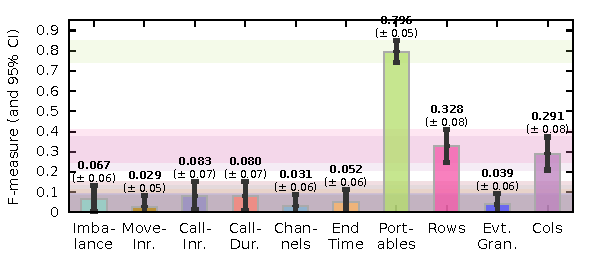
\includegraphics[width=\linewidth]{images/2tLadderQv3tHeapgsa_anal_shortPCS.pdf}\vspace{-0.1in}
\textbf{\caption{Summary of influential parameters from
Figure~\ref{fig:gsa-2tladv3tPCS} that cause performance differences
between \textbf{2tLadderQ} and \textbf{3tHeap} in sequential
simulations using PCS.}\label{fig:gsa-anal-2tladv3tPCS}}
\end{figure}
GSA to determine influential \textbf{PCS} parameters impacting the performance of
other scheduler queues against \textbf{2tLadderQ} showed that no parameter was more influential than \textbf{portables}. Furthermore, the results showed that \textbf{2tLadderQ} mostly outperformed the other scheduler queues with the exception of \textbf{2tHeap} and \textbf{3tHeap} in certain configurations.    

\subsection{Summary of GSA results for sequential simulations}\label{sec:seq-gsa-summary}

GSA shows that for comparing event queue performance in sequential simulations using our \textbf{PHOLD} benchmark and \textbf{PCS} simulation, we just need to focus on 1 or 2 parameters. Other aspects such as: event granularity, fraction of self-events, GVT rate, etc., do not matter for comparison of scheduler queues. The scheduler queues to focus further analysis are: \textbf{ladderQ}, \textbf{2tLadderQ}, and \textbf{3tHeap}.

\subsection{GSA results for parallel simulations}\label{sec:par-gsa}

GSA for parallel simulations were conducted using the same procedure discussed earlier but using 4 MPI-processes for parallel simulation. These analysis focused only on \textbf{ladderQ}, \textbf{2tLadderQ}, and \textbf{3tHeap} based on the inferences drawn from the earlier analyses. The average simulation execution time from 3 replications is recorded for each scheduler queue along with the parameter set.  For the parallel \textbf{PHOLD} simulation, we observed that the \textbf{ladderQ} timings showed a lot of variance in runtime depending on number of rollbacks that occur. Consequently, to reduce variance, we have used a time-window of 10 time-units to curtail optimism and reduce rollbacks.  The time-window restricts the simulation kernel from scheduling events that are more than 10 time-units ahead of GVT.  We use the same time-window for all
scheduler queues for consistent comparison and analysis. This consideration was not applied to the \textbf{PCS} simulation to remain consistent with the simulation properties as presented in \cite{carothers-94}.

\begin{figure}[H]
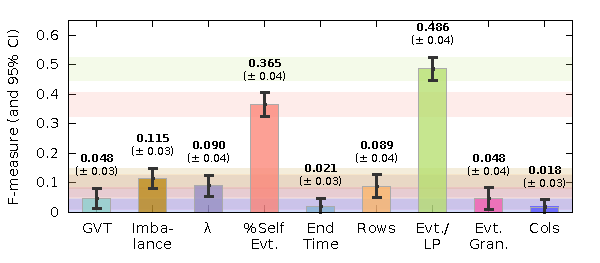
\includegraphics[width=\linewidth]{images/par_2tlad_vs_3tHeap_gsa_anal_short}\vspace{-0.1in}
\textbf{\caption{GSA data from parallel simulations (4 MPI-processes)
showing influential PHOLD parameters (\textbf{2tLadderQ}
vs. \textbf{3tHeap}).}\label{fig:par-gsa-anal-3tvs2t}}
\end{figure}


The chart in Figure~\ref{fig:par-gsa-anal-3tvs2t} shows the summary of the $d_{m,n}$ statistic or influence of each parameter (see
Table~\ref{tab:phold-params}) on the outcome -- \textit{i.e.,} \textbf{2tLadderQ} performs better or worse than \textbf{3tHeap}.  The lightly shaded bands show the 95\% Confidence Intervals (CI) computed using standard bootstrap approach using 5000 replications with 1000 samples in each. The parallel results are consistent with the sequential results and the \textbf{eventsPerLP} is the most influential parameter. However, in parallel simulation, the percentage of \textbf{selfEvents} (\textit{i.e.,} LPs schedule events to themselves) has a more pronounced influence when compared to $\lambda$.  The increased impact of \textbf{selfEvents} arises due to the use of optimistic synchronization. The self-events are local and can be optimistically processed, with some being rolled back, causing more operations on a larger pending event set. The data also shows that conspicuous \textbf{imbalance} in partitioning or load balance has some influence on the outcomes. However, in this study we explore typical parallel simulation scenarios in which load is reasonably well balanced.

\begin{figure}[H]
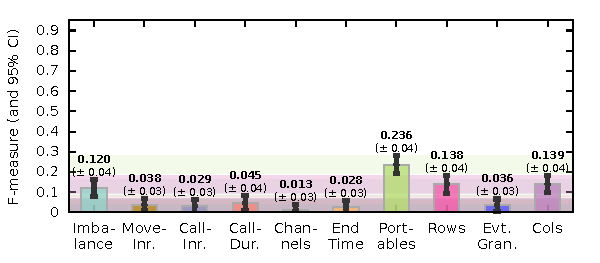
\includegraphics[width=\linewidth]{images/par2tLadderQv3tHeapgsa_anal_shortPCS.pdf}\vspace{-0.1in}
\textbf{\caption{GSA data from parallel simulations (4 MPI-processes)
showing influential PCS parameters (\textbf{2tLadderQ}
vs. \textbf{3tHeap}).}\label{fig:par-gsa-anal-3tvs2tPCS}}
\end{figure}

The chart in Figure~\ref{fig:par-gsa-anal-3tvs2tPCS} summarizes the $d_{m,n}$ statistic for parameters of the parallel \textbf{PCS} simulation (see Table~\ref{tab:pcs-params}). Once more \textbf{portables} is the most influential parameter with a subdued score of 0.236. Similarly, the model size has a marginal influence in the parallel simulation with scores of 0.138 and 0.139 for the model rows and columns. The \textbf{imbalance} parameter has a more pronounced effect in the parallel simulation but as previously mentioned, a well balanced scenario is presumed.    
\newpage
\section{Configurations for further analysis}\label{sec:configs}

\begin{table}[ht]\centering
\textbf{\caption{Configurations used for further analysis}\label{tab:configs}}
\begin{tabular}{llll}
\toprule
Name & \#LPs & \multicolumn{2}{c}{Sim. End Time} \\ \cline{3-4}
& (Rows\texttimes Cols) & Seq & Parallel \\
\midrule

\textbf{ph3} & 1,000 (100\texttimes 10) & 5000 & 20000 \\

\textbf{ph4} & 10,000  (100\texttimes 100) & 500 & 5000 \\

\textbf{ph5} & 100,000 (1000\texttimes 100) & 100 & 1000 \\

\midrule

\textbf{pcs6} & 100 (10\texttimes 10) & 5000 & 50000 \\

\textbf{pcs7} & 1,000  (100\texttimes 10) & 1000 & 4500 \\

\textbf{pcs8} & 10,000 (100\texttimes 100) & 100 & 200 \\

\bottomrule
\end{tabular}
\end{table}

The Generalized Sensitivity Analysis (GSA) enables identification of influential parameters, thereby substantially reducing the parameter
space. However, GSA data does not provide an effective data set to analyze trends, such as: scalability, memory usage, rollback
behaviors, etc. In order to pursue such analysis we have used 6 different configurations for the simulations. The \textbf{PHOLD} configurations are called \textbf{ph3}, \textbf{ph4}, and \textbf{ph5} and the \textbf{PCS} configurations are called \textbf{pcs6}, \textbf{pcs7}, and \textbf{pcs8}. The fixed characteristics for the 6 configurations is summarized in Table~\ref{tab:configs}. We use larger simulation end times for parallel simulation to obtain sufficiently long runtimes using 32 cores. The value of influential parameters, namely: \textbf{eventsPerLP}, \textbf{\%selfEvents}, and \textbf{$\lambda$} for the \textbf{PHOLD} configuration and \textbf{portables} for \textbf{PCS} is varied for comparing different settings, similar to the approach used by other investigators~\cite{tang-05,franceschini-15}.

\section{ \textbf{Sequential Simulations}}\label{sec:seq}

Sequential simulations were conducted to assess the effectiveness of the different data structures. We pursued sequential simulations to compare the base case performance of the data structures, consistent with prior investigations~\cite{tang-05,franceschini-15}. The sequential simulations also serve as a reference for potential use in conservatively synchronized PDES. The sequential experiments were conducted using 6 configurations listed in table~\ref{tab:configs} on one compute node of our cluster described in Section ~\ref{sec:platform}. The simulations use only 1 MPI-process and states are not saved. Number of sub-buckets in \textbf{2tLadderQ} was set to 1, \textit{i.e.,} \textsubscript{t2}\textit{k}=1. For the \textbf{PHOLD} experiments, the influential parameters \textbf{eventsPerLP}, $\lambda$, and \textbf{\%selfEvents} were varied to explore their impact on relative performance of the data structures. For the \textbf{PCS} experiments, the \textbf{portables} was the only influential parameter that was varied. Event \textbf{granularity} in both simulation models was set to zero resulting in a fine grained simulation. For each configuration, data from 10 independent replications were collected and analyzed.

\subsection{ \textbf{PHOLD sequential simulation results}}\label{sec:seq-phold}

The charts in Figure~\ref{fig:seq-time}(a)--(c) show change in runtime characteristics as the most influential parameter \textbf{eventsPerLP} is varied, for $\lambda$=1 (widest range of timestamps) and \textbf{\%self}\-\textbf{Events} = 0.25. This configuration was generally the best for \textbf{ladderQ}. As illustrated by Figure~\ref{fig:seq-time}(a)--(c), the performance of \textbf{ladderQ} and \textbf{2tLadderQ} (\textsubscript{2t}\textit{k}=1) is comparable as expected. However, the \textbf{2tLadderQ} performs slightly (paired \emph{t}-test p-value $<$ 0.05, \textit{i.e.,} averages are not equal) better in some cases possibly due to improved caching resulting from smaller tier-2 sub-buckets. These two queues outperform the other queues for lower values of \textbf{eventsPerLP}.

\begin{figure*}
\begin{minipage}{0.24\linewidth}
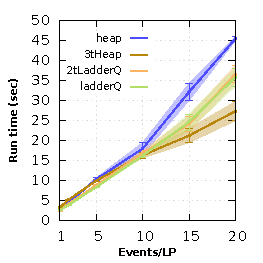
\includegraphics[width=\linewidth]{images/ph3_run_time}
\centerline{(a) \textbf{ph3}}
\end{minipage}
\begin{minipage}{0.24\linewidth}
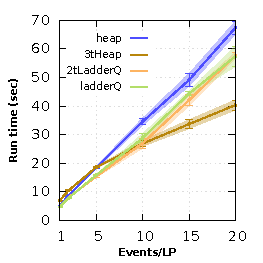
\includegraphics[width=\linewidth]{images/ph4_run_time}
\centerline{(b) \textbf{ph4}}
\end{minipage} 
\begin{minipage}{0.24\linewidth}
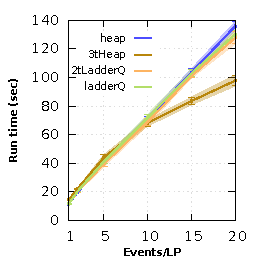
\includegraphics[width=\linewidth]{images/ph5_run_time}
\centerline{(c) \textbf{ph5}}
\end{minipage}
\begin{minipage}{0.24\linewidth}
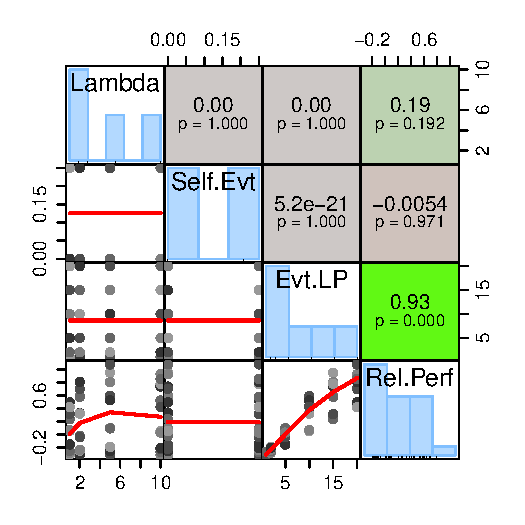
\includegraphics[width=\linewidth]{images/runtime_3tHeap_ladderQ_corr}
\centerline{(d) Corellogram}
\end{minipage}    

\textbf{\caption{Sequential simulation runtimes and correlation of
\textbf{3tHeap} performance with \textbf{PHOLD}
parameters}}\label{fig:seq-time}
\end{figure*}

However, the \textbf{3tHeap} generally outperforms the other queues (except for \textbf{2tHeap} in some cases) for higher values of \textbf{events\-Per\-LP}. In all cases, there were no inserts into \emph{Bottom} or \emph{Bottom}-to-\emph{Ladder} operations (discussed in Section~\ref{sec:fine-tune-lq}) that degrade \textbf{ladderQ} performance. The size of the \emph{Bottom} rung was proportional to the number of LPs and \textbf{eventsPerLP} -- \textit{i.e.,} with larger models, \emph{Bottom} has more events for many LPs with the same time stamp to be scheduled. In the larger configurations, the maximum of 8 rungs were fully used. The maximum rung threshold of 8 was determined to be an effective setting as discussed in Section~\ref{sec:fine-tune-lq} and the same value proposed by Tang et al~\cite{tang-05}.

Profiler data showed that the bottleneck in \textbf{ladderQ} arises from the overhead of re-bucketing events from rung-to-rung of the Ladder. On the other hand, in \textbf{3tHeap} re-bucketing does not occur. Consequently, the overheads of O(log $\frac{e}{c}$) operations in \textbf{3tHeap} are amortized as number of concurrent events $c$ increases.

The chart in Figure~\ref{fig:seq-time}(d) shows the correlation between the 3 influential parameters and the performance difference between \textbf{3tHeap} and \textbf{ladderQ}. Consistent with the GSA results, the correlogram shows that the most influential parameter is \textbf{eventsPerLP} (R=0.93, p=0) followed by $\lambda$ (R=0.19, p=0.192) with a very weak correlation. The \textbf{\%selfEvents} has practically no impact on performance. The correlogram also shows that these parameters are independent and have no covariance between each other
(R $\sim$ 0, p \textgreater 0.95).

\begin{figure}[H]
\begin{minipage}{0.32\linewidth}
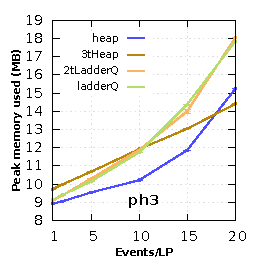
\includegraphics[width=\linewidth]{images/ph3_memory}
\end{minipage}
\begin{minipage}{0.32\linewidth}
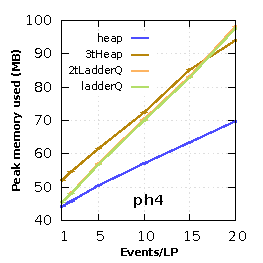
\includegraphics[width=\linewidth]{images/ph4_memory}
\end{minipage} 
\begin{minipage}{0.32\linewidth}
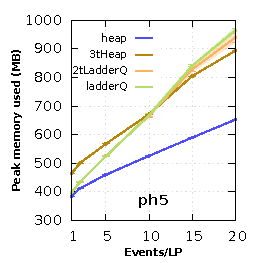
\includegraphics[width=\linewidth]{images/ph5_memory}
\end{minipage}
\textbf{\caption{Comparison of peak memory usage}\label{fig:seq-mem}}
\end{figure}

The charts in Figure~\ref{fig:seq-mem} shows the peak memory usage corresponding to the runtime data in Figure~\ref{fig:seq-time}. The
memory size reported is the ``Maximum resident set size'' value reported by GNU \textbf{/usr/bin/time} command on Linux. The memory usage
of \textbf{heap} is the lowest in most cases. Since \textsubscript{2t}\textit{k}=1, the memory usage of \textbf{ladderQ} and \textbf{2tLadderQ} is comparable as expected. The \textbf{3tHeap} initially uses more memory than the other data structures because of many small \textbf{std::vector}s and due to \textbf{std::vector} doubling its capacity.  However, the memory usage is amortized as the \textbf{eventsPerLP} increases. Consequently, the improved performance of \textbf{3tHeap} over \textbf{ladderQ} is realized without significant increase in memory footprint.
\newpage

\begin{figure*}[!htb]
\begin{minipage}{0.33\linewidth}
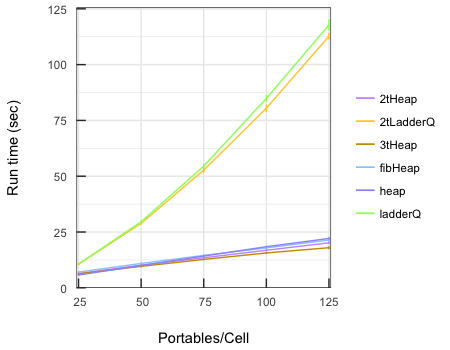
\includegraphics[width=\linewidth]{images/pcs6_runtime_full}
\centerline{(a) \textbf{pcs6}}
\end{minipage}
\begin{minipage}{0.33\linewidth}
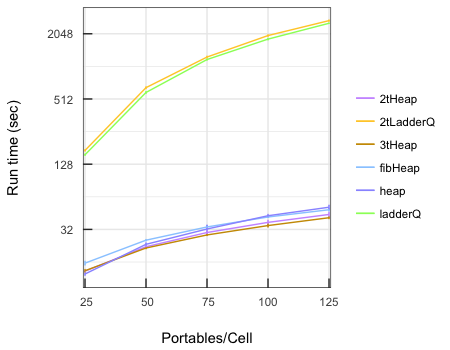
\includegraphics[width=\linewidth]{images/pcs7_runtime_full_log}
\centerline{(b) \textbf{pcs7}}
\end{minipage} 
\begin{minipage}{0.33\linewidth}
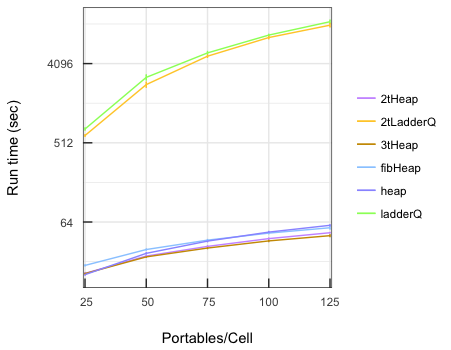
\includegraphics[width=\linewidth]{images/pcs8_runtime_full_log}
\centerline{(c) \textbf{pcs8}}
\end{minipage}
  
\textbf{\caption{Sequential simulation runtimes with PCS parameters}\label{fig:pcs-seq-time}}
\end{figure*}

\begin{figure*}[!htb]
\begin{minipage}{0.33\linewidth}
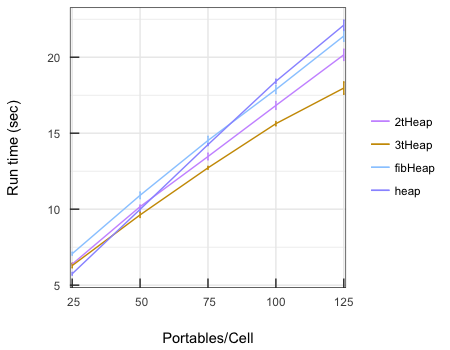
\includegraphics[width=\linewidth]{images/pcs6_runtime_partial2}
\centerline{(a) \textbf{pcs6}}
\end{minipage}
\begin{minipage}{0.33\linewidth}
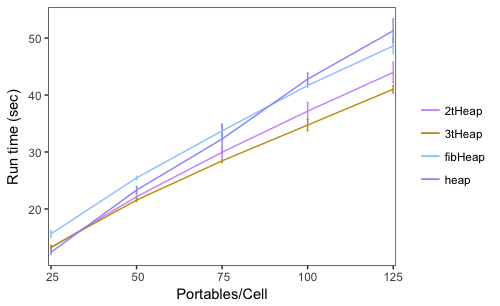
\includegraphics[width=\linewidth]{images/pcs7_runtime_partial2}
\centerline{(b) \textbf{pcs7}}
\end{minipage} 
\begin{minipage}{0.33\linewidth}
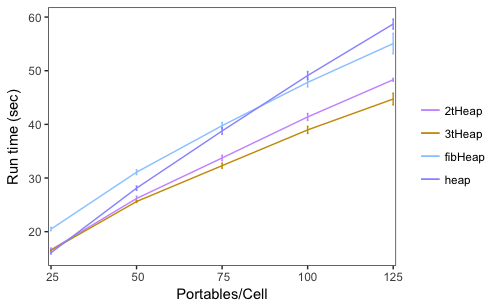
\includegraphics[width=\linewidth]{images/pcs8_runtime_partial2}
\centerline{(c) \textbf{pcs8}}
\end{minipage}
  
\textbf{\caption{Sequential simulation runtimes with PCS parameters}\label{fig:pcs-seq-time2}}
\end{figure*}

\begin{figure}[!htb]
\begin{minipage}{0.33\linewidth}
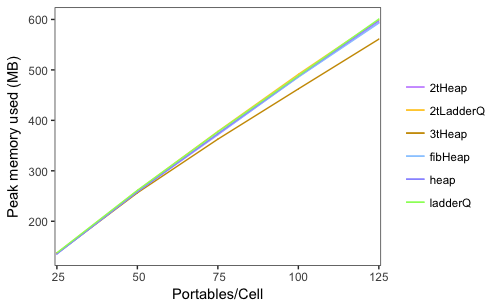
\includegraphics[width=\linewidth]{images/pcs6_memory_full}
\end{minipage}
\begin{minipage}{0.33\linewidth}
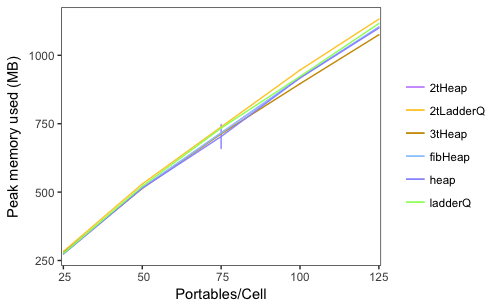
\includegraphics[width=\linewidth]{images/pcs7_memory_full}
\end{minipage} 
\begin{minipage}{0.33\linewidth}
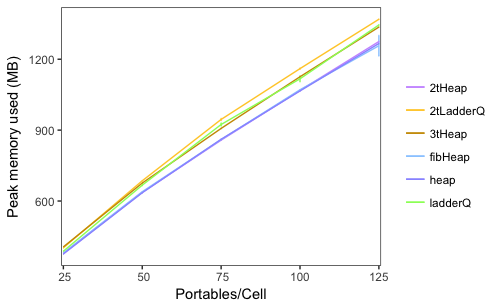
\includegraphics[width=\linewidth]{images/pcs8_memory_full}
\end{minipage}
\textbf{\caption{Comparison of peak memory usage}\label{fig:pcs-seq-mem}}
\end{figure}

\begin{figure*}\centering
\begin{minipage}{0.95\linewidth}
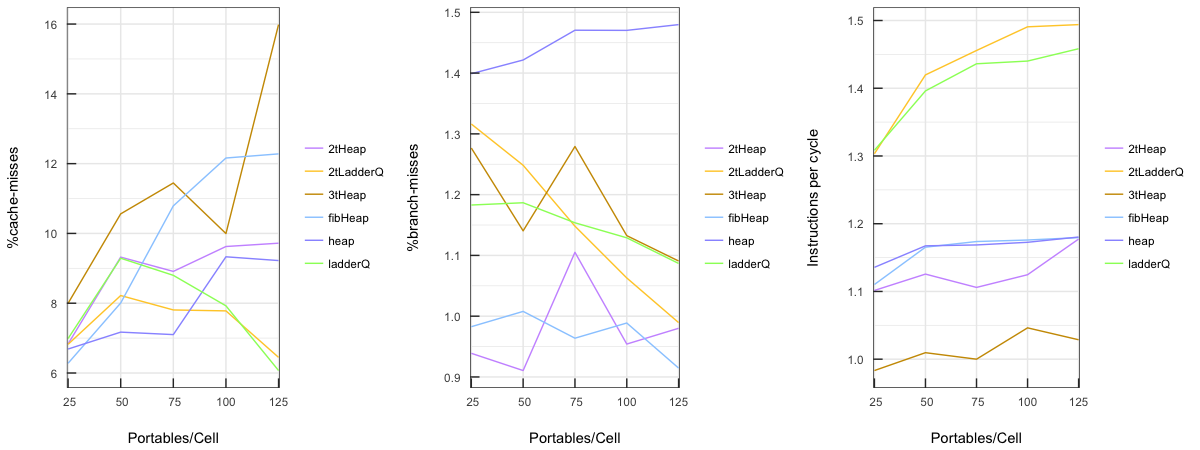
\includegraphics[width=\linewidth, height = 5cm]{images/pcs6_profile}
\centerline{(a) \textbf{pcs6}}
\end{minipage}
\begin{minipage}{0.95\linewidth}
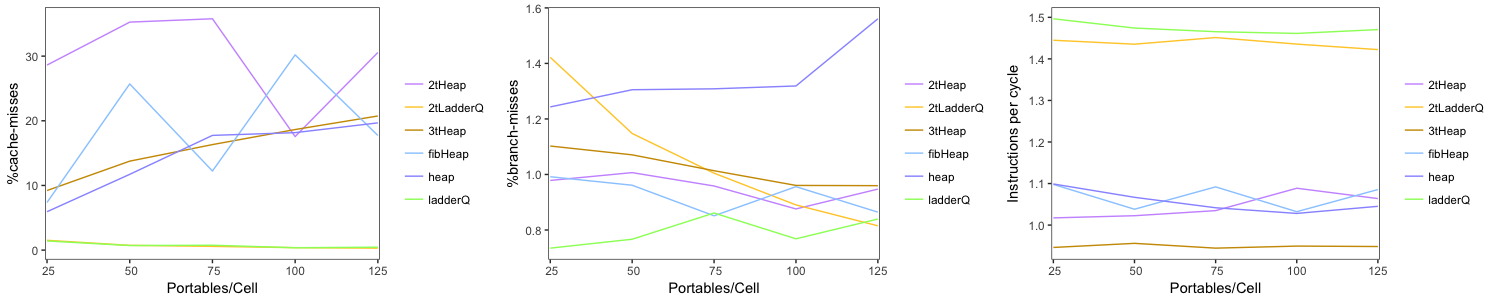
\includegraphics[width=\linewidth,  height = 5cm]{images/pcs7_profile}
\centerline{(b) \textbf{pcs7}}
\end{minipage} 
\begin{minipage}{0.95\linewidth}
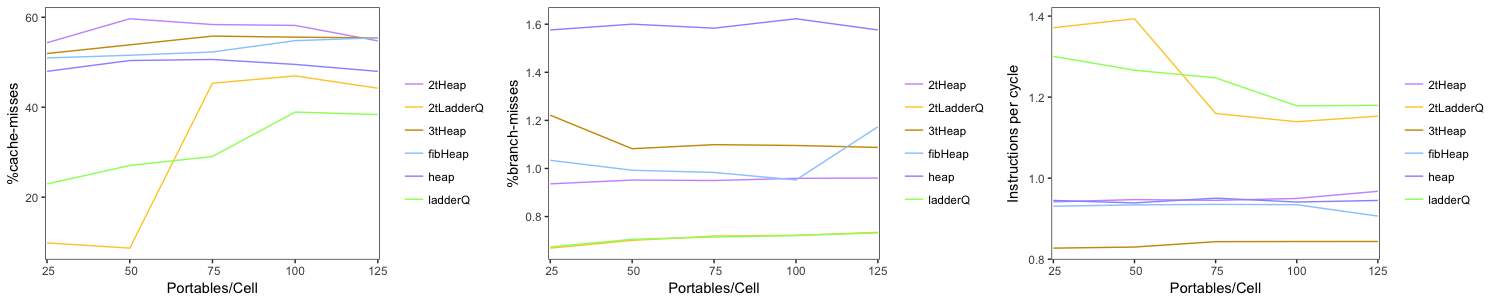
\includegraphics[width=\linewidth,  height = 5cm]{images/pcs8_profile}
\centerline{(c) \textbf{pcs8}}
\end{minipage}

\textbf{\caption{Profile results from PCS sequential simulation}\label{fig:pcs-profile}}
\end{figure*}


\subsection{\textbf{PCS} sequential simulation results}\label{sec:pcs_seq}

The charts in Figure\ref{fig:pcs-seq-time}(a)-(c) show runtime characteristics as the number of \textbf{portables} is varied using our 3 PCS configurations. As illustrated in the charts, the performance of \textbf{ladderQ} and \textbf{2tLadderQ} (\textsubscript{t2}\textit{k} = 1) is comparable. However, these two data structures were largely outperformed by the other scheduler queues. In fact, mean runtimes of \textbf{ladderQ} and \textbf{2tLadderQ} displayed an order of magnitude that was exceedingly high in comparison with the remaining queues. For the \textbf{pcs8} configuration with 125 \textbf{portables per cell}, the mean runtime values of the \textbf{ladderQ} and \textbf{2tLadderQ} were approximately 500\texttimes\/ higher than the runtime means of the other queues. Similarly to sequential simulation using the \textbf{PHOLD} benchmark, profile data from the \textbf{PCS} configurations showed that overhead of re-bucketing portables from rung-to-rung in both \textbf{ladderQ} and \textbf{2tLadderQ} degraded runtime performance. However, the impact of the overhead was even more pronounced in the \textbf{PCS} simulations.

The charts in Figure\ref{fig:pcs-seq-time2} (a)-(c) provide an illustration of the runtime performance of the scheduler queues without \textbf{ladderQ} and \textbf{2tLadderQ}. For the most part, \textbf{3tHeap} outperformed all of the other scheduler queues for higher number of \textbf{portables per cell}. As previously noted the re-bucketing operation is not a property of \textbf{3tHeap} and its design supports more efficient handling of an increasing number of concurrent events. 

The charts in Figure\ref{fig:pcs-seq-mem} show peak memory usage associated with runtime data displayed in Figures \ref{fig:pcs-seq-time} and \ref{fig:pcs-seq-time2}. The peak memory usage  is the lowest and tends to decrease with increasing number of \textbf{portables per cell} for \textbf{3tHeap} in configurations \textbf{pcs6} and \textbf{pcs7}. On the other hand \textbf{fibHeap} has the lowest memory usage in the \textbf{pcs8} configuration.

The charts in Figure\ref{fig:pcs-profile}(a)-(c) show profile results for the 3 configurations. As illustrated in the charts \textbf{ladderQ} and \textbf{2tLadderQ} displayed more effective use of the CPU data cache in all configurations, which is critical to performance. However, the percentage of instructions was also the highest for the two scheduler queues. This is consistent with the larger runtimes observed for \textbf{ladderQ} and \textbf{2tLadderQ}. On the other hand,\textbf{3tHeap} displayed a comparably higher percentage of cache and branch misses with respect to most of the scheduler queues, however, it also showed the lowest percentage of instructions in each configuration scenario. Thus, for sequential simulations using the \textbf{PCS} model, \textbf{3tHeap} is the desired scheduler queue for optimal runtime performance.

\section{\textbf{Parallel simulation assessments}}\label{sec:par}

The sequential simulation assessments indicated that \textbf{ladderQ}, \textbf{2tLadderQ}, and \textbf{3tHeap} performed the best for a broad range of \textbf{PHOLD} parameter settings. In particular, \textbf{3tHeap} performed the best for the \textbf{PCS} experiments. Consequently, we focused on assessing the effectiveness of these 3 queues for Time Warp synchronized parallel simulations. The experiments were conducted on our compute cluster (see Section ~\ref{sec:platform}) using a varying number of MPI-processes, with one process per CPU-core. In order to ensure sufficiently long runtimes with 32-cores, we increased \textbf{simEndTime} for parallel simulations as tabulated in Table~\ref{tab:configs}. The following subsections discuss results from the experiments.

\subsection{Throttling optimism with a time-window}

Initially we conducted experiments with fine-grained setting (\textit{i.e.,} \textbf{granularity} = 0) from sequential simulations. We noticed that the \textbf{ladderQ} had a large variance in runtimes, particularly when it experienced many rollbacks. In several cases, cascading rollbacks significantly slowed the simulations -- \textit{i.e.,} \textbf{ladderQ} simulations required over 1 hour while \textbf{2tLadderQ} would consistently finish in a few minutes. In order to avoid such debilitating rollback scenarios and to streamline experimental analysis timeframes we have throttled optimism using a time-window of 10 time-units. The time-window restricts the simulation kernel from scheduling events that are more than 10 time-units ahead of GVT. The time-window value of 10 is 50\% of the maximum timestamp of events generated by exponential distribution with $\lambda=1$. Consequently, most events in current schedule cycle will fit within this time-window with limited impact on concurrency. We use the same time-window for all scheduler queues for consistent comparison and analysis.

\subsection{Efficient case for \textbf{ladderQ}}

The charts in Figure~\ref{fig:par-time-1} show key simulation statistics for low value of \textbf{eventsPerLP} = 2 and $\lambda$=1 for
which \textbf{ladderQ} performed well, consistent with the observations in sequential simulations. The statistics show average and 95\% CI
computed from 10 independent replications for each data point. The peak rollbacks among all of the MPI-processes is shown as it controls
overall progress in the parallel simulations. As illustrated by the data in Figure~\ref{fig:par-time-1}, both the \textbf{ladderQ} and
\textbf{2tLadderQ} perform well for all three models. In this configuration, overall the \textbf{ladderQ} experienced the fewest
rollbacks. Nevertheless, the \textbf{2tLadderQ} continues to perform well despite experiencing more rollbacks as shown in
Figure~\ref{fig:par-time-1}(b). The good performance of \textbf{2tLadderQ} under heavy rollback is consistent with its design objective to enable rapid event cancellation and improve rollback recovery. The maximum of 8 rungs on the ladder was reached in all the simulations, but with only few (1 to 3) buckets per rung. On average, the number of \emph{Bottom} to Ladder operations (that degrade performance) were low
per MPI process, about -- \textbf{ph3}: \{9144, 8911\}, \textbf{ph4}: \{1904, 1448\}, and \textbf{ph5}: \{53, 84\} for \{\textbf{ladderQ}, \textbf{2tLadderQ}\} respectively. We did not observe a strong correlation between number of these operations and rollbacks.

\begin{figure*}
\begin{minipage}{0.32\linewidth}
\begin{minipage}{0.49\linewidth}
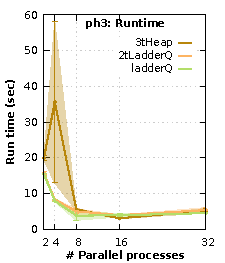
\includegraphics[width=\linewidth]{images/ph3_Delay_1_Evt_2_run_time}
\end{minipage}
\begin{minipage}{0.49\linewidth}
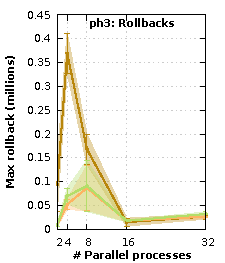
\includegraphics[width=\linewidth]{images/ph3_Delay_1_Evt_2_rollbacks}
\end{minipage}
\centerline{(a) \textbf{ph3} time \& rollbacks}
\end{minipage}
\begin{minipage}{0.32\linewidth}
\begin{minipage}{0.49\linewidth}
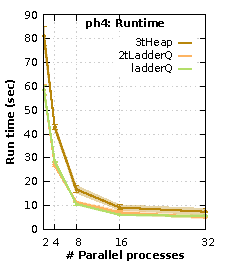
\includegraphics[width=\linewidth]{images/ph4_Delay_1_Evt_2_run_time}
\end{minipage}
\begin{minipage}{0.49\linewidth}
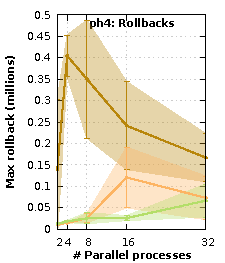
\includegraphics[width=\linewidth]{images/ph4_Delay_1_Evt_2_rollbacks}
\end{minipage}
\centerline{(b) \textbf{ph4} time \& rollbacks}    
\end{minipage}
\begin{minipage}{0.32\linewidth}
\begin{minipage}{0.49\linewidth}
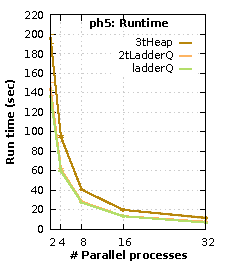
\includegraphics[width=\linewidth]{images/ph5_Delay_1_Evt_2_run_time}
\end{minipage}
\begin{minipage}{0.49\linewidth}
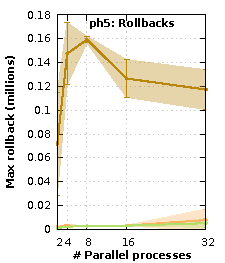
\includegraphics[width=\linewidth]{images/ph5_Delay_1_Evt_2_rollbacks}
\end{minipage}
\centerline{(c) \textbf{ph5} time \& rollbacks}    
\end{minipage}
\textbf{\caption{Statistics from PHOLD parallel simulation with \textbf{eventsPerLP}=2, $\lambda=1$, \textbf{\%selfEvents}=25\%}\label{fig:par-time-1}}
\end{figure*}

In this configuration, the \textbf{3tHeap} runs experienced a lot of rollbacks when compared to the other two queues despite the time-window. For \textbf{ph5} data in Figure~\ref{fig:par-time-1}(c), \textbf{3tHeap} experienced about 114805 rollbacks on average while \textbf{ladderQ} experienced only 2341, almost 50\texttimes fewer rollbacks. Consequently, it was slower than the other 2 queues, but its performance is not significantly degraded -- \~1.5\texttimes\/ slower despite 50\texttimes\/ more rollbacks. The peak memory usage for all the 3 queues was comparable in these
configurations.

\subsection{Knee point for \textbf{3tHeap} vs. \textbf{ladderQ}}

The charts in Figure~\ref{fig:par-time-2} show key simulation statistics for the configuration where \textbf{3tHeap} and \textbf{ladderQ}
performed about the same in sequential (see Figure~\ref{fig:seq-time}).  For \textbf{ph3}, both \textbf{ladderQ} and \textbf{2tLadderQ} experienced comparable number of rollbacks but the \textbf{2tLadderQ} performs better due to its design advantages. In the case of \textbf{ph4} and \textbf{ph5}, both the \textbf{ladderQ} and \textbf{3tHeap} experienced a comparable number of rollbacks, but much higher than the \textbf{2tLadderQ} despite having a time-window. Nevertheless, the \textbf{3tHeap} conspicuously outperforms the \textbf{ladderQ} because it is able to quickly cancel events and complete rollback processing. For \textbf{ph5}, the \textbf{3tHeap} outperforms the other 2 queues despite the high number of rollbacks. The peak memory usage for all the 3 queues was comparable in these configurations.

\begin{figure*}
\begin{minipage}{0.32\linewidth}
\begin{minipage}{0.49\linewidth}
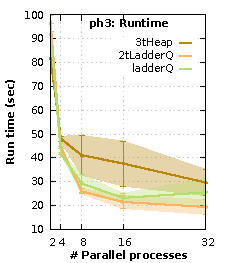
\includegraphics[width=\linewidth]{images/ph3_Delay_10_Evt_10_run_time}
\end{minipage}
\begin{minipage}{0.49\linewidth}
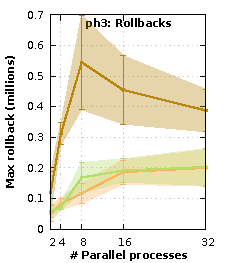
\includegraphics[width=\linewidth]{images/ph3_Delay_10_Evt_10_rollbacks}
\end{minipage}
\centerline{(a) \textbf{ph3} time \& rollbacks}
\end{minipage}
\begin{minipage}{0.32\linewidth}
\begin{minipage}{0.49\linewidth}
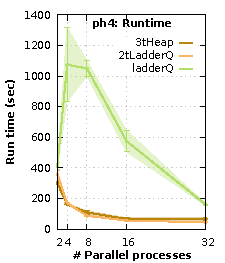
\includegraphics[width=\linewidth]{images/ph4_Delay_10_Evt_10_run_time}
\end{minipage}
\begin{minipage}{0.49\linewidth}
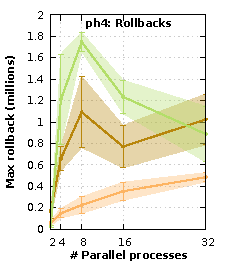
\includegraphics[width=\linewidth]{images/ph4_Delay_10_Evt_10_rollbacks}
\end{minipage}
\centerline{(b) \textbf{ph4} time \& rollbacks}    
\end{minipage}
\begin{minipage}{0.32\linewidth}
\begin{minipage}{0.49\linewidth}
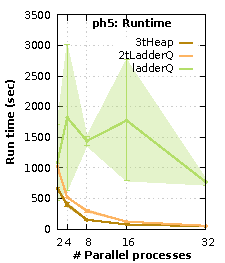
\includegraphics[width=\linewidth]{images/ph5_Delay_10_Evt_10_run_time}
\end{minipage}
\begin{minipage}{0.49\linewidth}
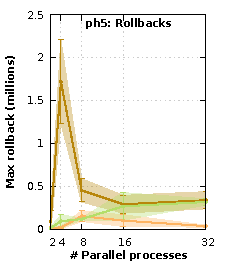
\includegraphics[width=\linewidth]{images/ph5_Delay_10_Evt_10_rollbacks}
\end{minipage}
\centerline{(c) \textbf{ph5} time \& rollbacks}    
\end{minipage}  
\textbf{\caption{Statistics from PHOLD parallel simulation with \textbf{eventsPerLP}=10, $\lambda=10$, \textbf{\%selfEvents}=25\%}\label{fig:par-time-2}}
\end{figure*}

\begin{figure}[H]\centering
\begin{minipage}{0.25\linewidth}
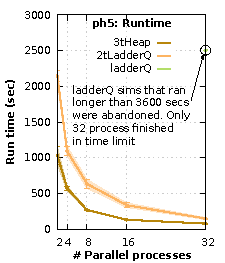
\includegraphics[width=\linewidth]{images/ph5_Delay_10_Evt_20_run_time}
\end{minipage}
\begin{minipage}{0.25\linewidth}
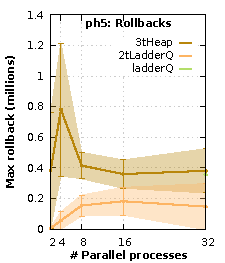
\includegraphics[width=\linewidth]{images/ph5_Delay_10_Evt_20_rollbacks}
\end{minipage}
\textbf{\caption{\textbf{ph5} Statistics (best case for \textbf{3tHeap})}\label{fig:par-time-3}}
\end{figure}


\begin{figure*}\centering
\begin{minipage}{0.80\linewidth}
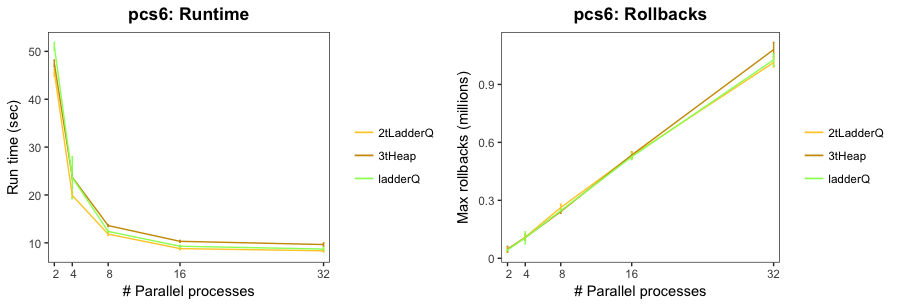
\includegraphics[width=\linewidth]{images/pcs6_parallel_25}
\centerline{(a) \textbf{pcs6} time \& rollbacks}
\end{minipage}
\begin{minipage}{0.80\linewidth}
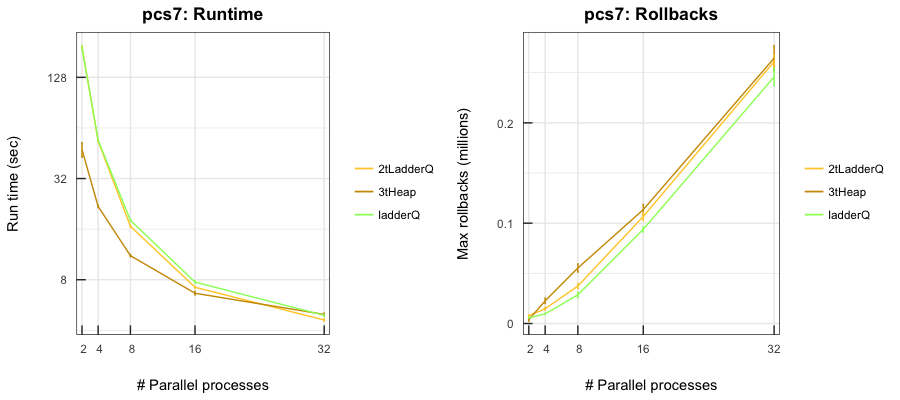
\includegraphics[width=\linewidth]{images/pcs7_parallel_25_log}
\centerline{(b) \textbf{pcs7} time \& rollbacks}
\end{minipage} 
\begin{minipage}{0.80\linewidth}
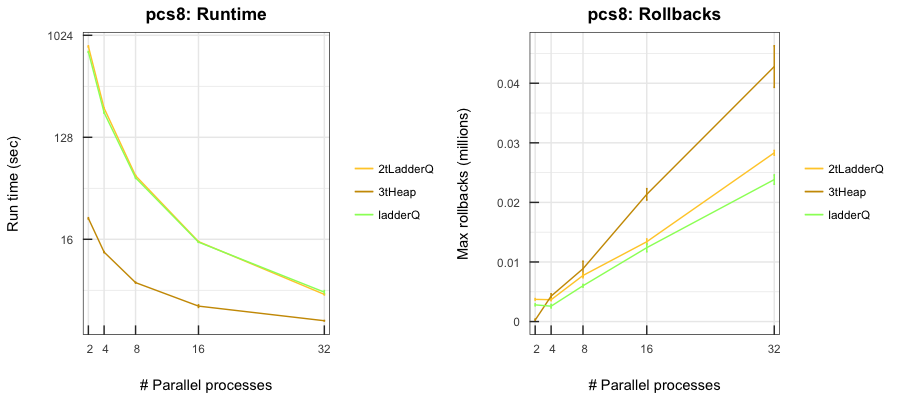
\includegraphics[width=\linewidth]{images/pcs8_parallel_25_log}
\centerline{(c) \textbf{pcs8} time \& rollbacks}
\end{minipage}

\textbf{\caption{Statistics from PCS parallel simulation with \textbf{portables}=25}\label{fig:pcs-par-time-1}}
\end{figure*}

\begin{figure*}\centering
\begin{minipage}{0.80\linewidth}
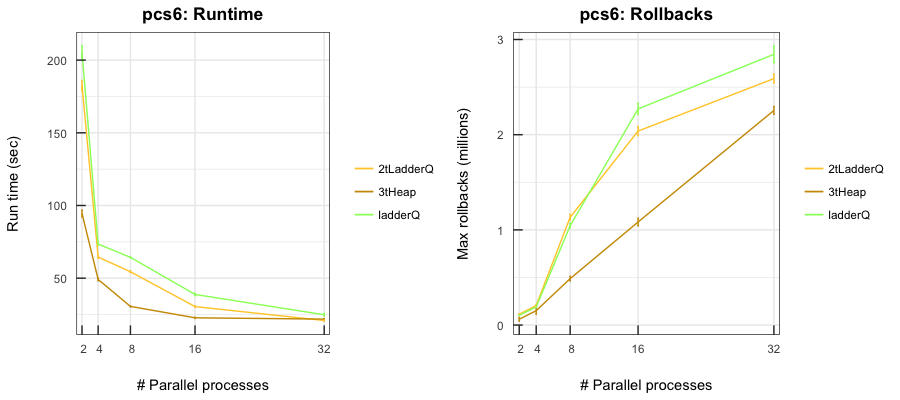
\includegraphics[width=\linewidth]{images/pcs6_parallel_75}
\centerline{(a) \textbf{pcs6} time \& rollbacks}
\end{minipage}
\begin{minipage}{0.80\linewidth}
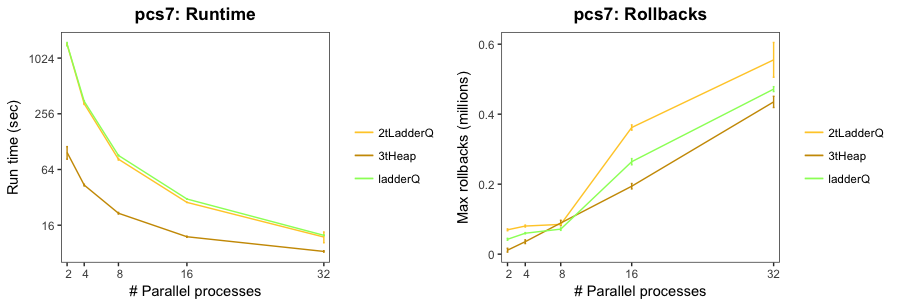
\includegraphics[width=\linewidth]{images/pcs7_parallel_75_log}
\centerline{(b) \textbf{pcs7} time \& rollbacks}
\end{minipage} 
\begin{minipage}{0.80\linewidth}
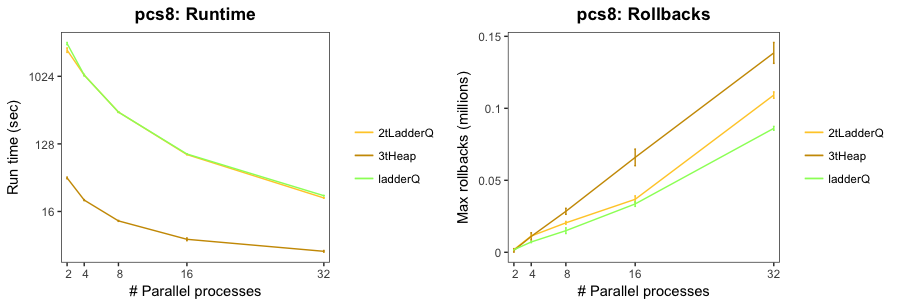
\includegraphics[width=\linewidth]{images/pcs8_parallel_75_log}
\centerline{(c) \textbf{pcs8} time \& rollbacks}
\end{minipage}

\textbf{\caption{Statistics from PCS parallel simulation with \textbf{portables}=75}\label{fig:pcs-par-time-2}}
\end{figure*}

\subsection{Best case for \textbf{3tHeap}}

Figure~\ref{fig:par-time-3} shows simulation time and rollback characteristics in high concurrency configuration with \textbf{ph5}, with
\textbf{eventsPerAgent}=20, $\lambda$=10, and \textbf{\%Self Evt.}=25\%. The \textbf{ladderQ} runs exceeded 3600 seconds in most cases even with a time-window, except for 32 processes. Consequently \textbf{ladderQ} experiments with fewer than 32 processes were abandoned. On the other
hand \textbf{2tLadderQ} performed well due to its design. The \textbf{3tHeap} outperformed the other 2 queues despite experiencing ~2\texttimes\/
more rollbacks.

Figures ~\ref{fig:pcs-par-time-1} and ~\ref{fig:pcs-par-time-2} show parallel simulation runtime and rollback characteristics with \textbf{pcs6}, \textbf{pcs7} and \textbf{pcs8} for \# of \textbf{portables} set equal to 25 and 75, respectively. Generally, \textbf{3tHeap} outperformed the other scheduler queues for all configurations. The performance benefits of \textbf{3tHeap} was more noticeable in the \textbf{pcs8} configuration while undergoing a greater number of rollbacks, as illustrated in Figures ~\ref{fig:pcs-par-time-1}(c) and ~\ref{fig:pcs-par-time-2}(c). In the \textbf{pcs8} configuration with 75 \textbf{portables per cell} and 32 processors, \textbf{3tHeap} experienced an average of 203624 rollbacks, while \textbf{2tLadderQ} experienced 137800 and \textbf{ladderQ} experienced 90540 rollbacks. 

